%%===========================================================%%
%%                                                           %%
%%                       FORWARD PROTONS                     %%
%%                                                           %%
%%===========================================================%%


\chapter{Forward protons}\label{chap:forwardProtons}

\section{Roman Pot track reconstruction}

\subsection{Alignment}

\section{Roman Pot simulation}

\begin{figure}[hb]%
\caption[Apertures.]{Apertures.}\label{fig:aperturesWithFit}%
\centering
\parbox{0.495\textwidth}{
  \centering
  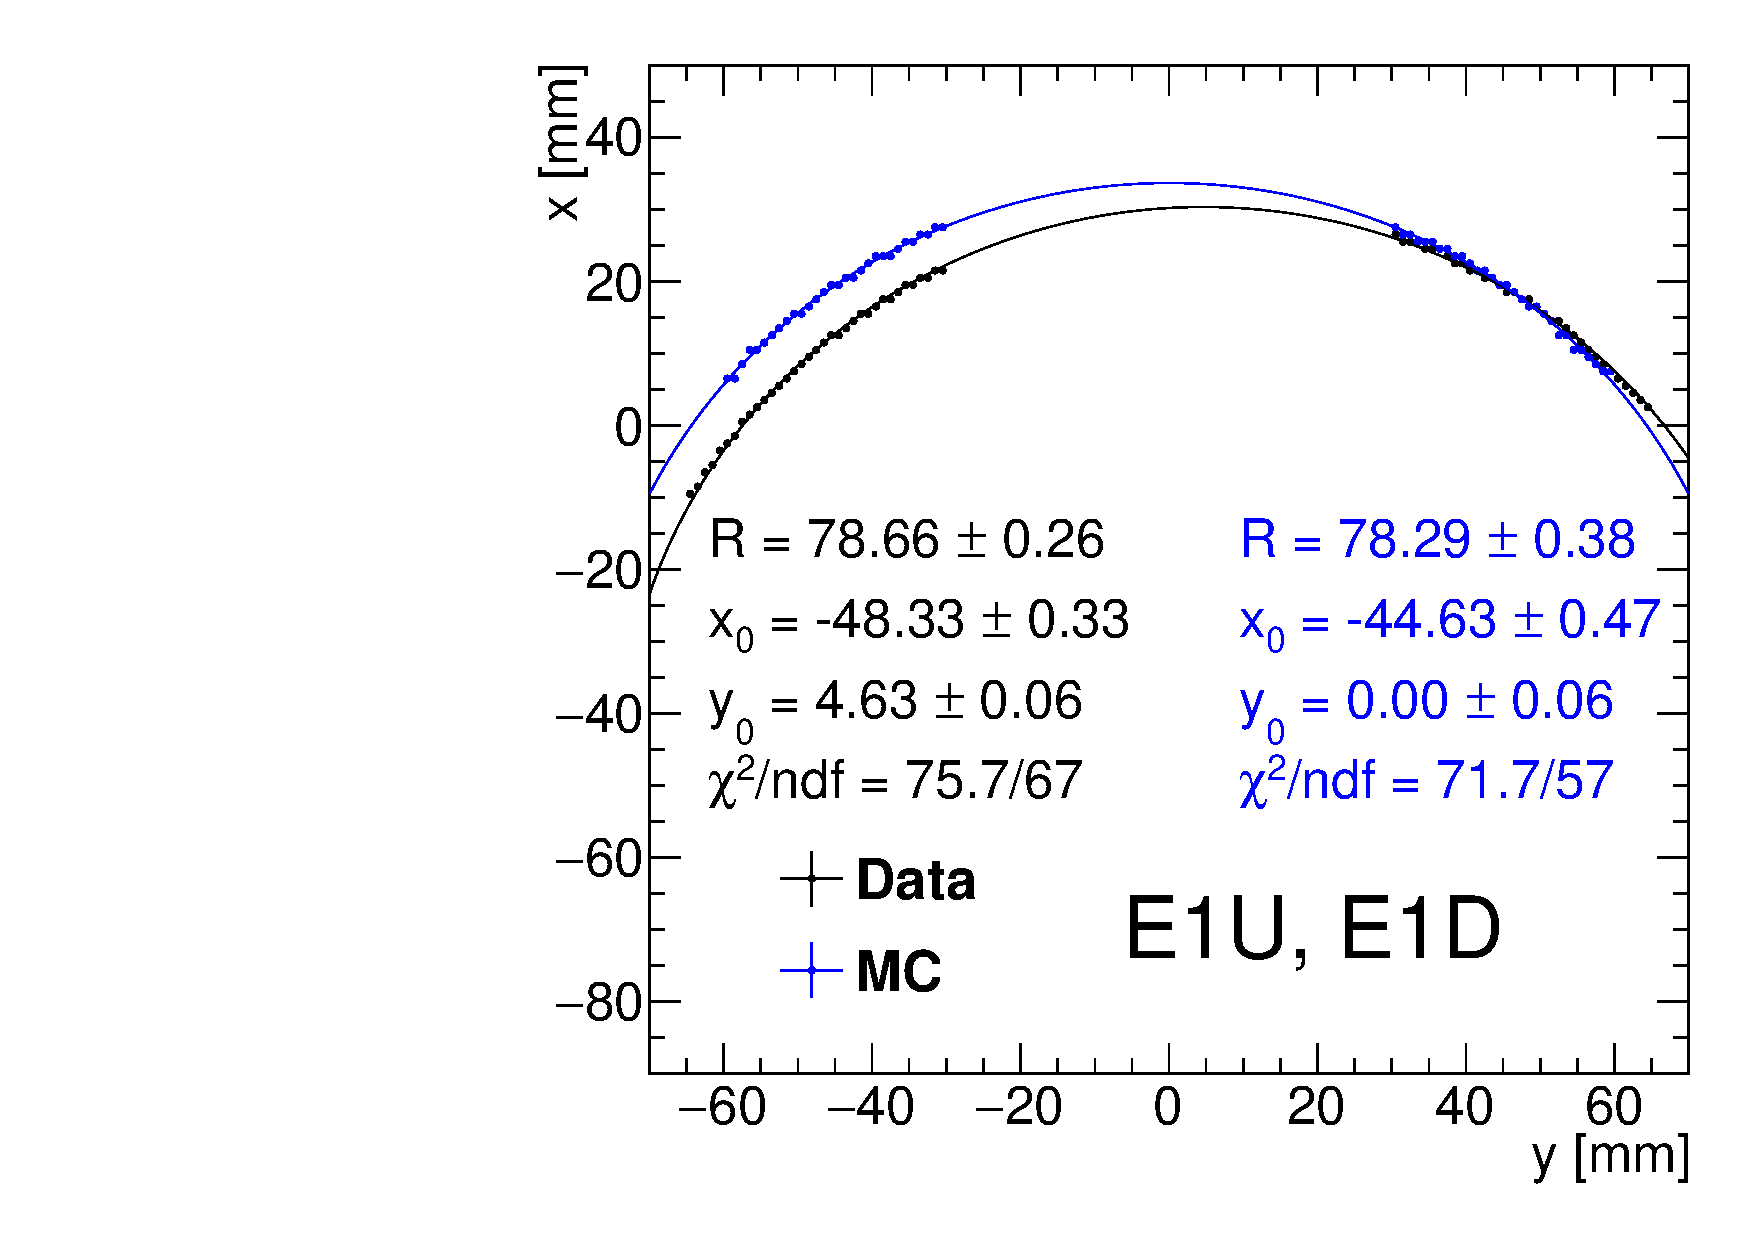
\includegraphics[width=\linewidth,page=1]{graphics/rpSim/Apertures_swapedAxes_withFit_beforeDxShift.pdf}\\
  \includegraphics[width=\linewidth,page=2]{graphics/rpSim/Apertures_swapedAxes_withFit_beforeDxShift.pdf}\\
  \includegraphics[width=\linewidth,page=3]{graphics/rpSim/Apertures_swapedAxes_withFit_beforeDxShift.pdf}
}~
\parbox{0.495\textwidth}{
  \centering
  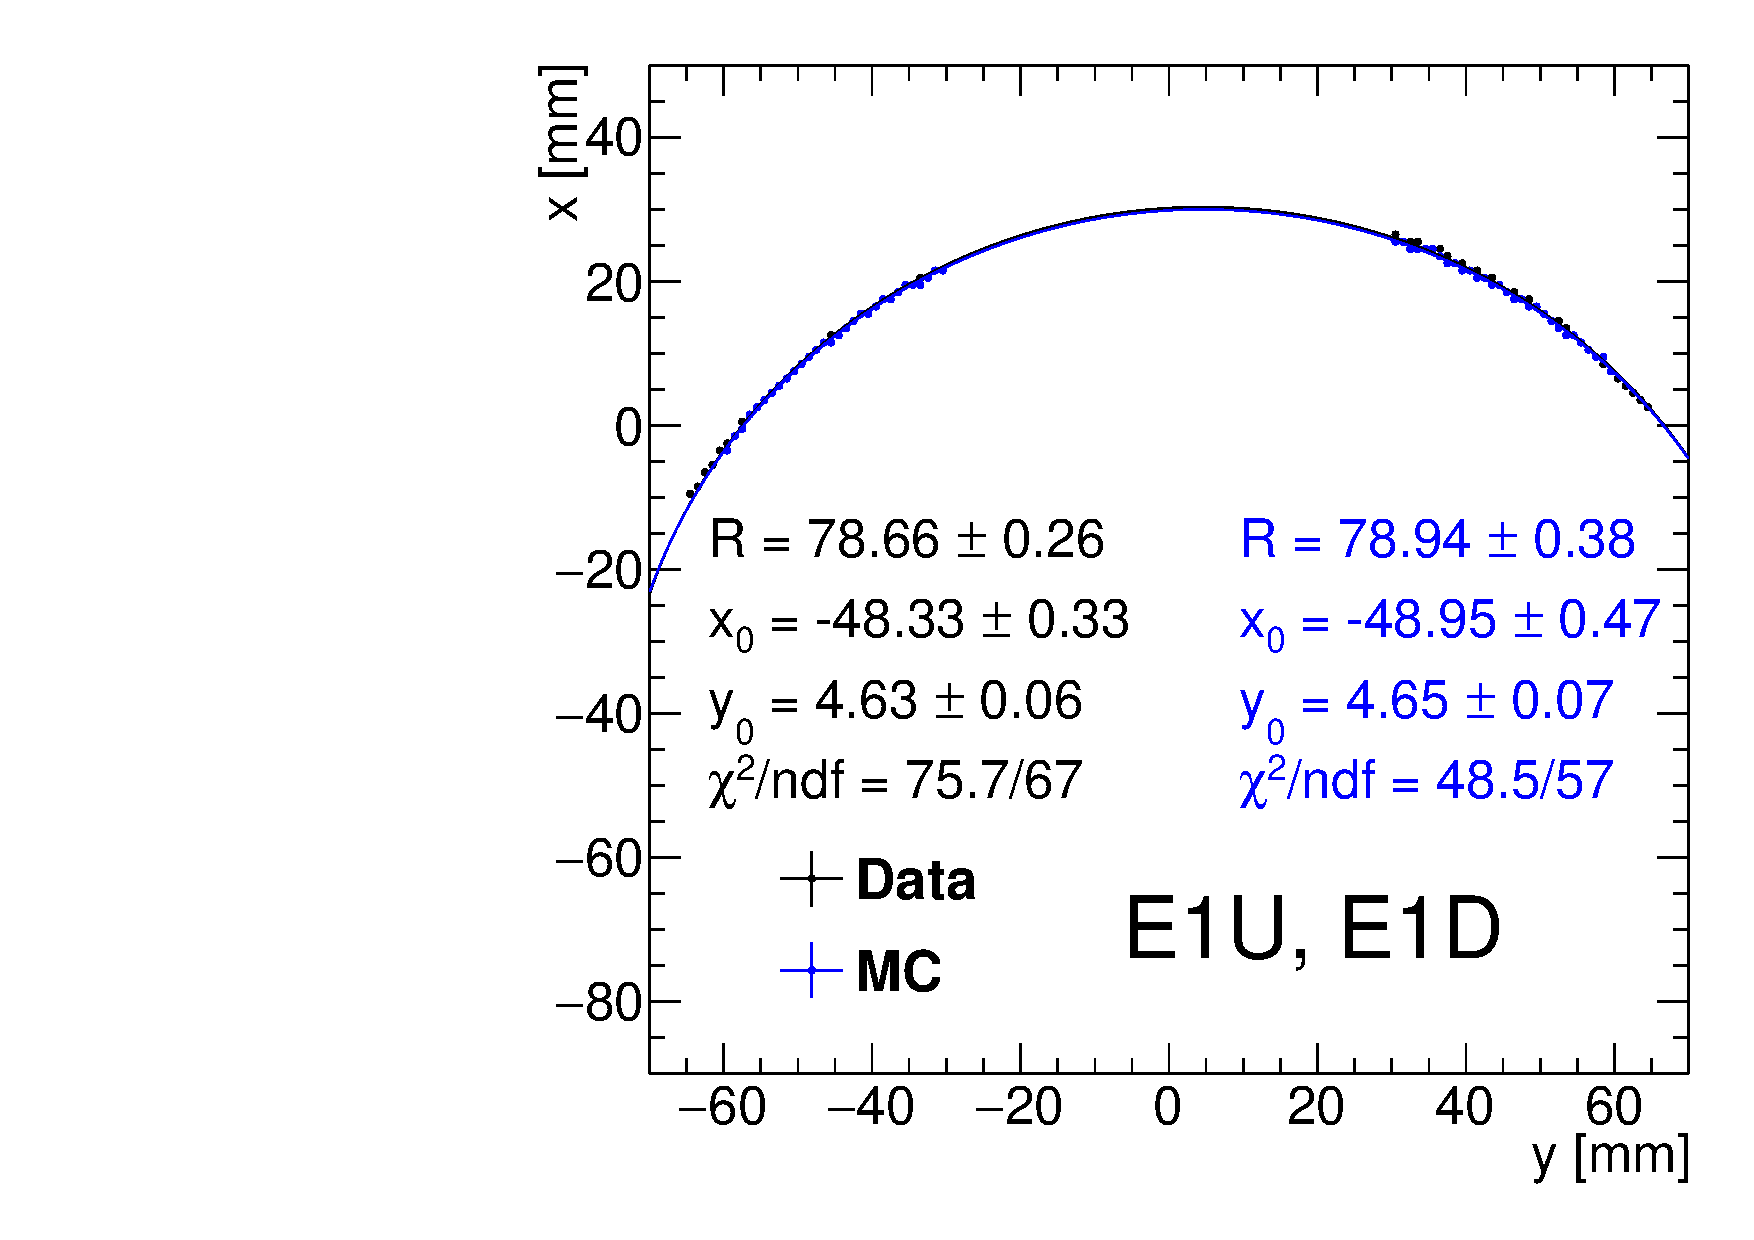
\includegraphics[width=\linewidth,page=1]{graphics/rpSim/Apertures_swapedAxes_withFit.pdf}\\
  \includegraphics[width=\linewidth,page=2]{graphics/rpSim/Apertures_swapedAxes_withFit.pdf}\\
  \includegraphics[width=\linewidth,page=3]{graphics/rpSim/Apertures_swapedAxes_withFit.pdf}
}%
\end{figure}
\begin{figure}[ht!]\ContinuedFloat
% ~\\[32pt]
\centering
\parbox{0.495\textwidth}{
  \centering
  \includegraphics[width=\linewidth,page=4]{graphics/rpSim/Apertures_swapedAxes_withFit_beforeDxShift.pdf}
}~
\parbox{0.495\textwidth}{
  \centering
  \includegraphics[width=\linewidth,page=4]{graphics/rpSim/Apertures_swapedAxes_withFit.pdf}
}%
\end{figure}
%---------------------------